\chapter{Implementation}
In this chapter we will briefly outline the approach we took for the implementation of the Schafkopf environment and
the training pipeline.


\section{Enviroment}
The environment was programmed in Python for its fast development and integration of current Reinforcement libraries
such as PyTorch, and follows the traditional Model-View-Controller(\textbf{MVC}) paradigm.
\textbf{MVC} is an established concept for game environments as it cleanly separates the game logic held in the
model
with the decision process making of the controller in our case the agents interacting with the environment.
In our implementation there are two main components necessary to play a hand of Schafkopf:
\begin{description}
    \item[Game Object] Acts as the model and handles the game logic, game phases and action validation
    \item[Player Object] Acts as the controller and makes an agents individual decision based on the implemented logic
\end{description}

\subsection{Game Object}
The game object is initialised with a list of four agent objects, a lead variable that determines the player position
with the \textbf{Lead} role.
Optionally a seed variable can be passed to control
Internally it follows the game phases defined in \ref{gamephases} .\\
In the\textbf{ Setup phase} it creates a shuffled 32 card deck and deals each player eight cards.
The deck's order can optionally be controlled via a seed variable, which can be useful for debugging or replaying
certain games for evaluation, for example if we want only seeds that give players \textbf{Solo} cards.
\newline
During \textbf{Bidding phase} each player in their respective order at the virtual table is given their hand in
combination with their valid bidding options, which depend on previous bids as well as their hand, by calling the
players' bidding methods.
Once every player has returned their bid the \textbf{Bidding phase} concludes, the highest bid and resulting game
mode can be
determined.
If at this stage no contract has been decided the hand ends immediately.
The hand moves now into the \textbf{Trick phase} after variables such as team composition, run away possibilities and
other game mode induced variables have been evaluated.
\newline
In \textbf{Trick phase} for each of the eight tricks we perform the same loop of actions starting with the leading
player:
\begin{enumerate}
    \item Set the players current hand in the corresponding player object
    \item Determine the valid cards the player may play
    \item Pass the game state,current trick history and valid cards to player by calling player's \textit{playCard}
    method
    \item Check if the action returned by the player is valid
\end{enumerate}
After all players played their card, the trick winner is determined, the point scores are updated, and played cards
are removed from the corresponding hands.
After \textbf{Team Mode} it is also important to check if players \textbf{ran away}} or \textbf{searched} as this is
vital to allow for correct deduction of valid cards that can be played.
\newline
Once all eight tricks have been played successfully the \textbf{Scoring phase} commences and a winner and resulting
reward is calculated and the hand is concluded.
\subsection{Game State}
The game state holds all information that define a hand at any moment and is held and passed as dictionary throughout
the environment.
\newline
\begin{table}[h!]
\begin{tabular}{lll}
Name              & Type           & Description                                                             \\
\hline
Hands             & List of Cards  & Description                                                             \\
Game Mode         & Category       & Can be one of eigth possible contracts                                  \\
Lead              & Int            & Table position of leading player                                        \\
Scores            & List of Int    & List of length four                                                     \\
Trick History     & Tuple of Cards & Tuples that keep track of pass tricks                                   \\
Cards Played      & List of Cards  & List of all the cards played (Not necessary, but useful for perfomance) \\
Seed              & Int            & Records the Seed for debugging and evaluation                           \\
Offensive Players & Int            & List of table positions of bid winner and partner                       \\
Run Away Possible & Bool           & Can partner technically run away                                        \\
Ran Away          & Bool           & Did partner run away                                                    \\
Searched          & Bool           & Has been searched
\end{tabular}
\caption{Game state and its members.}
\label{tab:gamestate}
\end{table}

\subsection{Player Class}
The player class is a template class \ref{lst:playerclass} that every agent inherits from.
It handles an agent's decision process during the bidding phase as well as the trick phase.
The two main methods that any agent has to shadow are \textit{makebid()} and \textit{playCard()}.
These are called by the environment and make the agent the controller in the \textbf{MVC} paradigm.
\newline
\begin{lstlisting}[!H][language=Python,label={lst:playerclass}]
import random
class Player():
def __init__(self, name):
self.name = name
self.hand = []
self.position = None

def setHand(self, cards):
self.hand = []
self.hand = cards

def setPosition(self, postion):
self.position = postion

def makeBid(self, validBids):
return random.choice(validBids)

def playCard(self, validCards, gameState, trickHistory):
return random.choice(validCards)
\end{lstlisting}
\section{Reinforcement Learning Setup}
The common reinforcement learning libraries(OpenAI and RLlib) either did either not support multi-agent learning
environments or turn-based game types, so we decided on implementing the learning setup in PyTorch.
The actual training was performed on Google Colab, even though our training was not very GPU intensive, it proved
useful to avoid crashing local machines on long training runs with large batch sizes.
\subsection{PPO}
The \textbf{PPO} implementation used was taken and adapted from a similar project on GitHub \cite{emerich}
This allowed to set hyper-paramaters, such as learning rate, clipping values, decay, batch size.
\subsection{One-Hot Encoding}
To encode the game state into a vector we encoded all necessary information using One-hot encoding.
Cards and hands were encoded using a 32 bit vector, where each index represents a unique card.\\
The index of a card can be calculated using \[index(card) = Suit * 8 + rank\].
When positions are passed they are always a 4 bit vector where index 0 is the player.
This way all information, like bid winner and current lead, is always from the ego perspective.
\subsection{Player experiences}
To update our network we need to collect the experiences of each player during their exploration of the game
environment.
We collect at each step in the hand:
\begin{description}
\item[Action] The sampled action that was taken
\item[Log Probabilities] The probability distribution of our action space
\item[State] The input state
\item[Terminal] True if the action was terminal (last trick), otherwise False
\item[Reward] Final Reward of the hand
\end{description}
Due to the nature of Schafkopf, rewards are only received at the end of each episode.
We use reward discounting to assign rewards to non-terminal states as well by multiplying the terminal reward with a
discount factor (0.99 was used). See the code below for the method used.
\begin{lstlisting}[!h][language=Python,label={lst:rewards},caption={Reward calculation for non-terminal steps}]
rewards = []
gamma = 0.99
discountedReward = 0
for reward, isTerminal in zip(rewards), terminal)):
if isTerminal:
discountedReward = 0
discountedReward = reward + (self.gamma * discountedReward)
rewards.append(discountedReward)
\end{lstlisting}
With this we can create for each hand eight Markov decision tuples: \[(S,A,P_{a},R_{a})\]\\
These make up our training data for our PPO update.
Since we use self play with four identical agents we actually get 32 tuples for each hand we play during self-play.

\subsection{Training Pipeline}
The training pipe line always follows the same procedure for each episode:
\begin{enumerate}
\item Load the latest model
\item Play hands with
\item Collect Experiences from each player
\item Update the network using PPO
\item Run evaluation against baseline agents
\item Log results for evaluation and for update
\item Save the updated network
\end{enumerate}



\section{Reinforcement Learning Agents}
The models we trained are simple {\textbf{feed forward NN} that receive a game state, which is processed and then fed
through the Network to produce two outputs: 32x1 vector that gives us our probabilities of all the valid
actions (\textit{actor}), and 1x1 vector which describes our state-value function (\textit{critic}). (See Fig
.\ref{fig:layerchart})\\
All inner layers use 48 hidden \textbf{ReLÚ} neurons
Overall we trained two agents, \textbf{CompleteRL} and \textbf{SeperatedRL}, that both use the same actor-critc network
design.
\begin{figure}[!h]
\centering
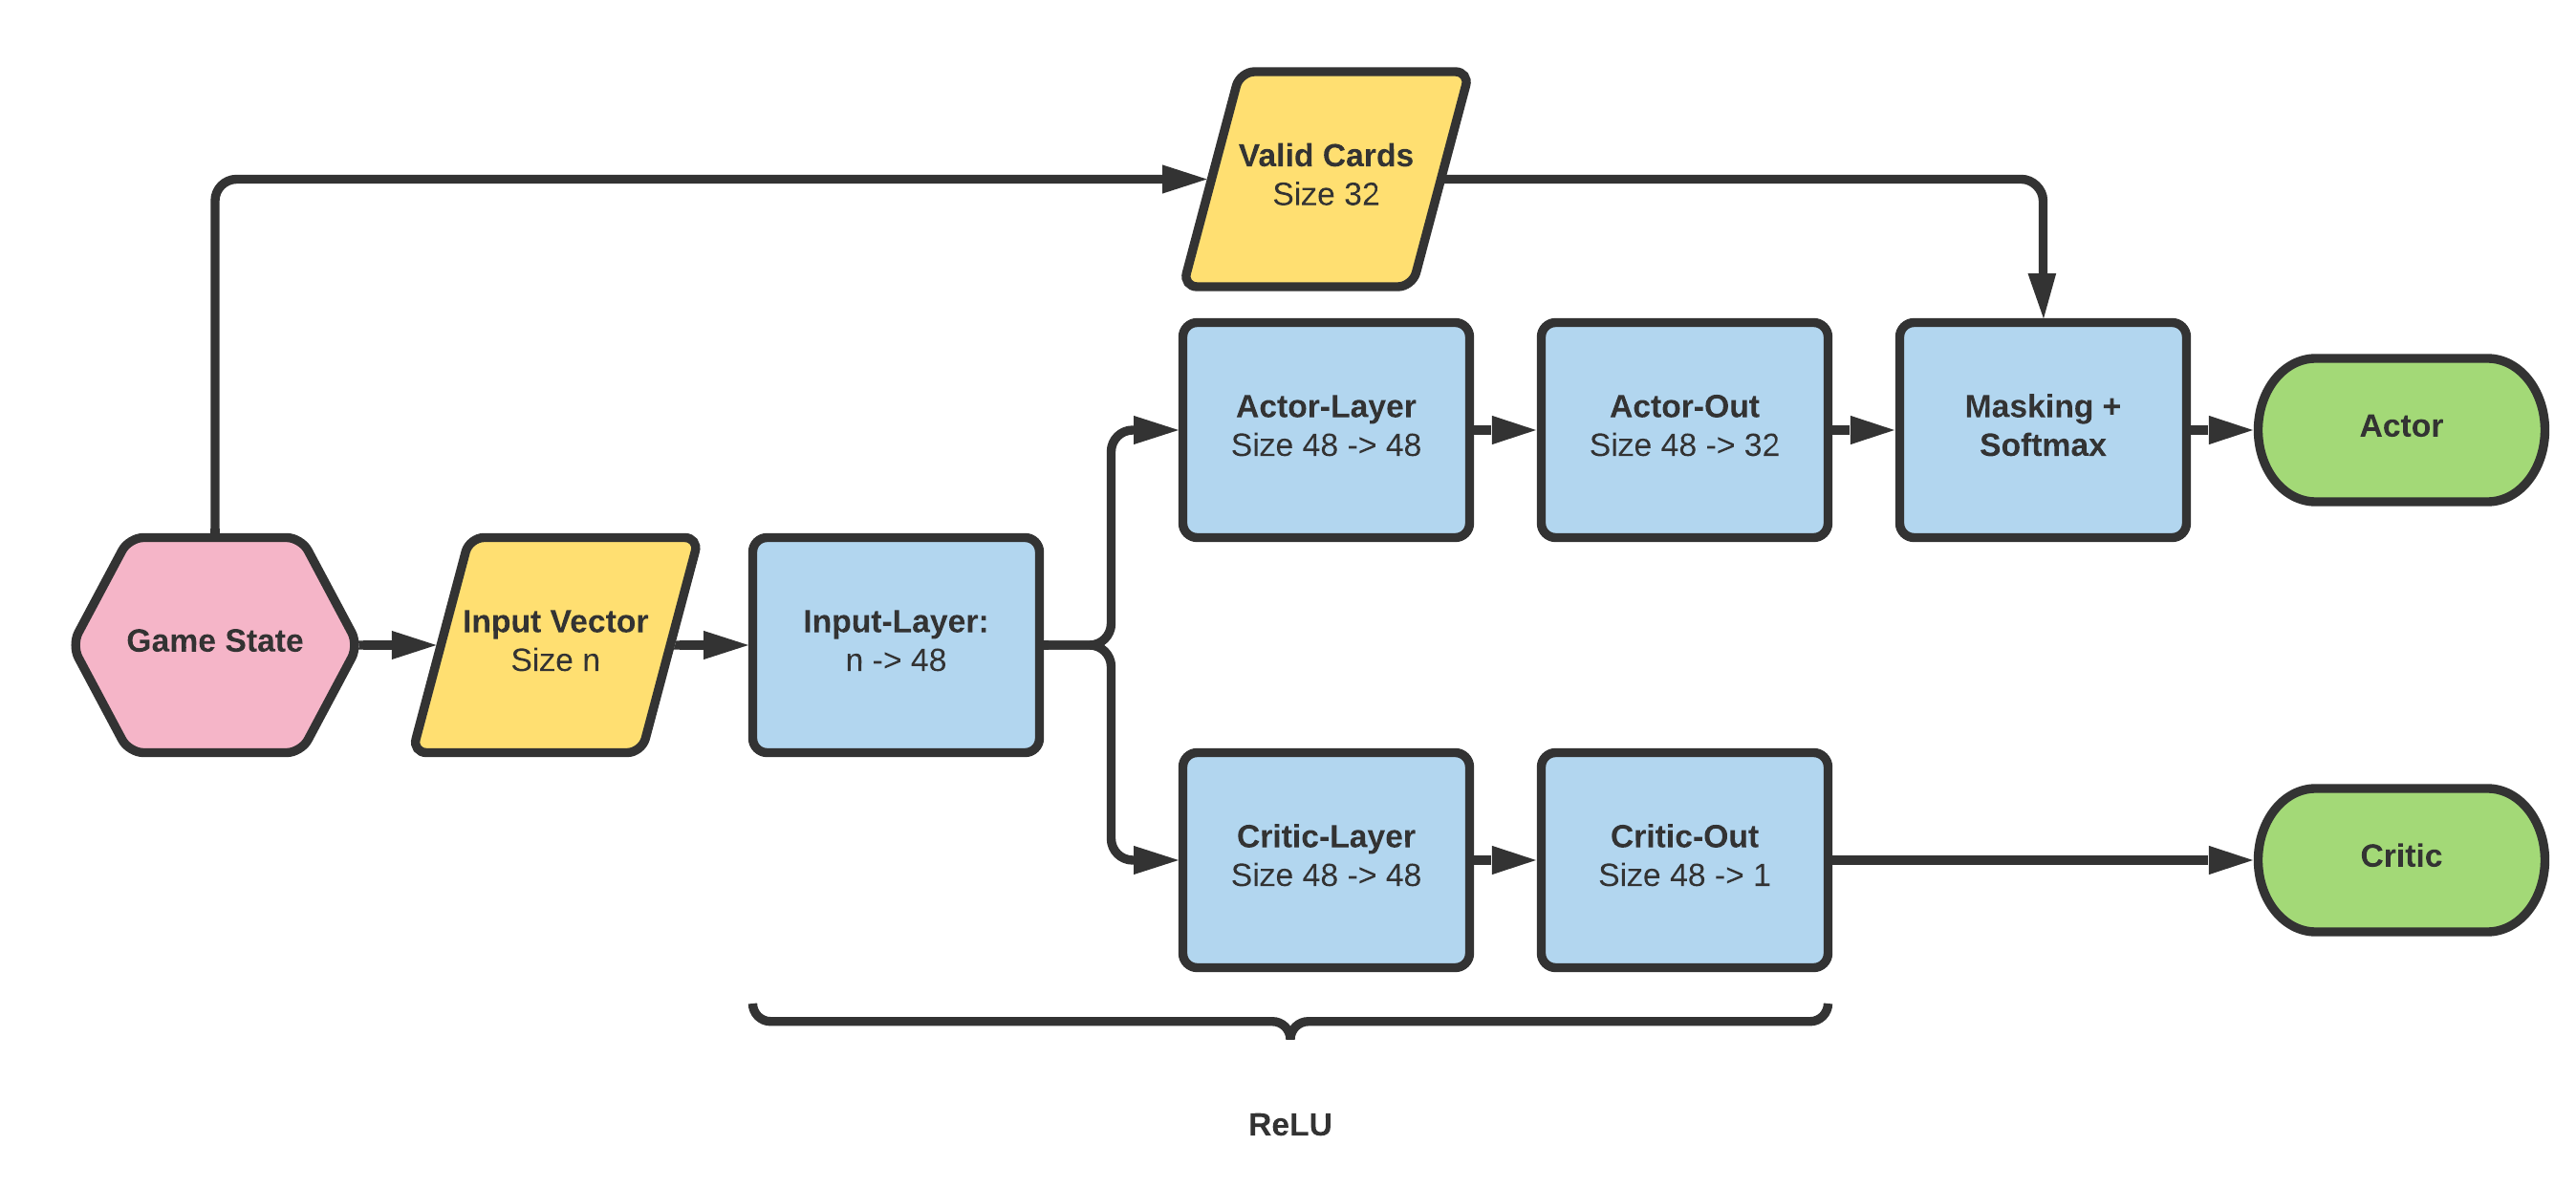
\includegraphics[width=\textwidth]{layerchart.png}
\caption{Network layer flow used the Actor-Critic Models}
\label{fig:layerchart}
\end{figure}
\end{center}
\subsection{CompleteRL}
The CompleteRL agent uses the same network for all three game modes.
This was our initial approach, to see if one network can do it all.
The input vector (See Tab. \ref{tab:CompleteRLinput}), derived from the game state, uses \textit{one hot encoding}
for all cards, positions and information and is always rotated so the acting player is in position zero, to keep the
vector representation
consistent.\\
\begin{table}[!h]
\centering
\begin{tabular}{lll}
\toprule
Name          & Size     & Description                                           \\
\midrule
Hand          & 32       & Hand of the player                                    \\
Cards Played  & 32       & All cards in previous tricks                          \\
Lead          & 4        & Position that started the trick                       \\
Game Mode     & 7        & 3 contracts + 4 colours                               \\
Ran Away      & 1        & If partner ran away (Bool)                            \\
Searched      & 1        & If the ace has been searched (Bool)                   \\
Bid Winner    & 4        & Position that won the bidding                         \\
Own Team      & 4        & Position of own Team (1000 if unknown)                \\
Scores        & 4*1      & Scores for each position (Normalised using Score/120) \\
Trick History & (32+4)*4 & Cards played by each position                        \\
\midrule
Sum & 233 & Total size of the input Vector\\
\bottomrule
\end{tabular}
\caption{Input vector for the CompleteRL model}
\label{tab:CompleteRLinput}
\end{table}

\subsection{SeperatedRL}
As an experiment we also trained \textbf{SeperatedRL} that has a different model for each of the three contracts
(Team,Wenz,Solo).
The idea is to reduce the variance in the training data, whilst also only including the relevant information and thus
slimming the input vector.
The major drawback of this is naturally training time, but we reduced the batch size during training compared to
\textbf{SeperatedRL} but tried to keep learning steps when evaluation the two.

\begin{table}[!h]
\centering
\begin{tabular}{lllll}
\toprule
Name          & \multicolumn{3}{c}{Size}                                               & Description
\\
\midrule
& Team     & Wenz                      & Colour-Solo                     &
\\
\midrule
Hand          & 32       & 32                        & 32                              & Hand of the player
\\
Cards Played  & 32       & 32                        & 32                              & All cards in previous tricks
\\
Lead          & 4        & 4                         & 4                               & Position that started the
trick                       \\
Game Mode     & 4        & 0 & 4                               & 4 colours
\\
Ran Away      & 1        & 0 & 0       & If partner ran away (Bool)                            \\
Searched      & 1        & 0 & 0       & If the ace has been searched (Bool)                   \\
Bid Winner    & 4        & 4                         & 4                               & Position that won the
bidding                         \\
Own Team      & 4        & 4                         & 4                               & Position of own Team (1000
if unknown)                \\
Scores        & 4*1      & 4*1                       & 4*1                             & Scores for each position
(Normalised) \\
Trick History & (32+4)*4 & (32+4)*4                  & (32+4)*4} & Cards played by each position
\\
\midrule
Sum           & 214      & 208                       & 212                             & Total size of the input
Vector\\
\bottomrule
\end{tabular}
\caption{Input vector for each sub model of the SeperateRL agent}
\label{tab:Seperatedinput}
\end{table}

